\documentclass{article}
\usepackage{geometry}
\usepackage{graphicx}
\usepackage{subcaption}
\usepackage{placeins}
\usepackage{hyperref}
\usepackage{url}

\title{BME 599: Advanced Topics in MRI\\HW \#2}
\author{Tom Griesler}

\geometry{left=2cm, right=2cm, top=1cm}

\date{\today}
\begin{document}

\maketitle

\section*{Problem 1: Extended phase graphs.}
% \textbf{Shown below is a sequence diagram of a fast spin echo (FSE) with its first 8 refocusing pulses within one repetition time (TR). Each RF pulse is designated as a delta function, so you do not need worry about the slice profile. Refocusing pulses are spaced 5ms apart (echo spacing).}

\begin{itemize}

    \item[a.] %Please write a function using EPG to simulate spin echo train echo amplitudes for a sequence with $90$°$_x$ excitation, followed by refocusing pulses of $[\alpha+(90- \alpha/2)]_y$ , $\alpha_y$, $\alpha_y$ ,... for 64 echoes for $T1 = [200:100:1500]\,$ms, and $T2 = [50:30:300]\,$ms
    
        \begin{itemize}

            \item[i.] cf. Figure \ref{fig:1_a_i} %Simulate echo amplitudes with $\alpha = 180$°, and plot amplitudes with five different T1 and T2 combinations
            
                \begin{figure}[]
                    \centering
                    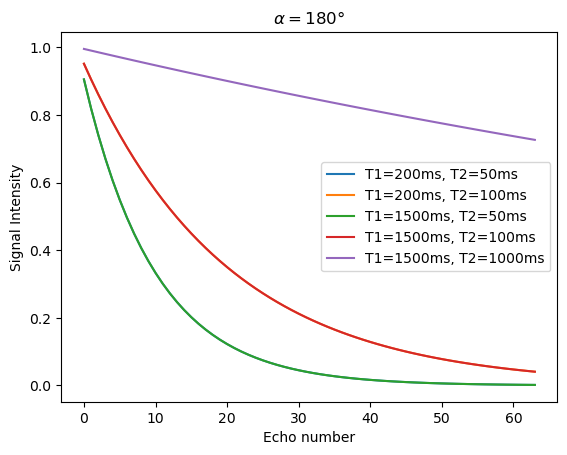
\includegraphics[width=0.7\textwidth]{figures/1_a_i.png}
                    \caption{Echo amplitudes with $\alpha=180$°.}
                    \label{fig:1_a_i}
                \end{figure}

            \item[ii.] cf. Figure \ref{fig:1_a_ii} %Simulate echo amplitudes with $\alpha = 120$°, and plot amplitudes with five different T1 and T2 combinations
            
                \begin{figure}[]
                    \centering
                    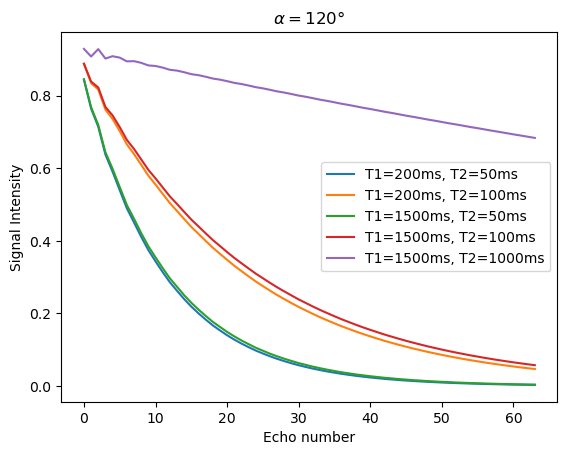
\includegraphics[width=0.7\textwidth]{figures/1_a_ii.png}
                    \caption{Echo amplitudes with $\alpha=120$°.}
                    \label{fig:1_a_ii}
                \end{figure}
            
            \item[iii.] cf. Figure \ref{fig:1_a_iii} %Simulate echo amplitudes with $\alpha = 60$°, and plot amplitudes with five different T1 and T2 combinations
            
                \begin{figure}[]
                    \centering
                    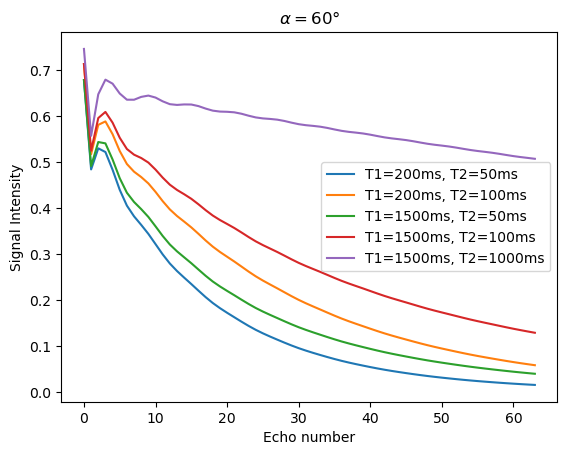
\includegraphics[width=0.7\textwidth]{figures/1_a_iii.png}
                    \caption{Echo amplitudes with $\alpha=60$°.}
                    \label{fig:1_a_iii}
                \end{figure}

        \end{itemize}

    \item[b.] An exemplary contour plot of the signal vs. T1 and T2 at the 6th echo when using 180° refocusing pulses is shown in Figure \ref{fig:1_b}. %Plot 4 contour plots signals vs T1 and T2 for the 6th, 16th, 32nd, and 48th echoes using various $\alpha$
    
    \begin{figure}[]
        \centering
        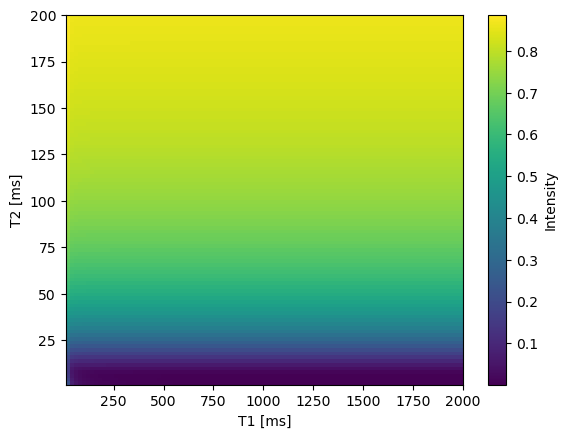
\includegraphics[width=0.7\textwidth]{figures/1_b.png}
        \caption{Contour plot of the signal intensity at the 6th echo when using $180$° refocusing pulses.}
        \label{fig:1_b}
    \end{figure}
    
    \item[c.] %Discuss the contrast you get with different flip angles.
    
    When using $180$° pulses, the contrast solely depends on T2. With lower refocusing flip angles, the contrast starts to additionally depend on T1. 

\end{itemize}

\section*{Problem 2: Single and Multiple Spin Echo Sequences.}

\begin{itemize}
    \item[a. ] \textbf{Single-echo spin echo.}
    Figures \ref{fig:2_a_t1}, \ref{fig:2_a_t2}, and \ref{fig:2_a_pd} show the T1, T2 and PD weighted simulated SE images. 

    \begin{figure}[]
        \centering
        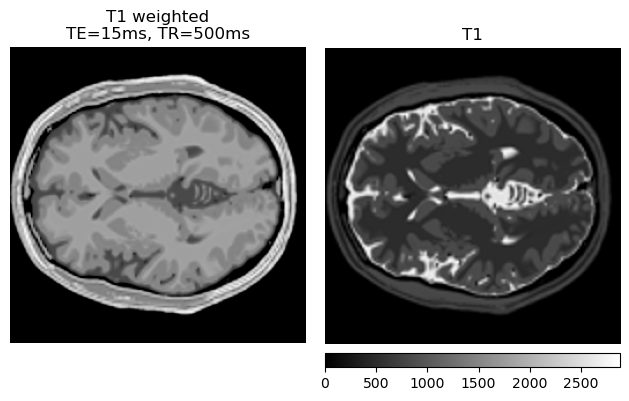
\includegraphics[width=0.8\textwidth]{figures/2_a_t1.png}
        \caption{Simulated T1 weighted SE image (left) compared to T1 map (right).}
        \label{fig:2_a_t1}
    \end{figure}

    \begin{figure}[]
        \centering
        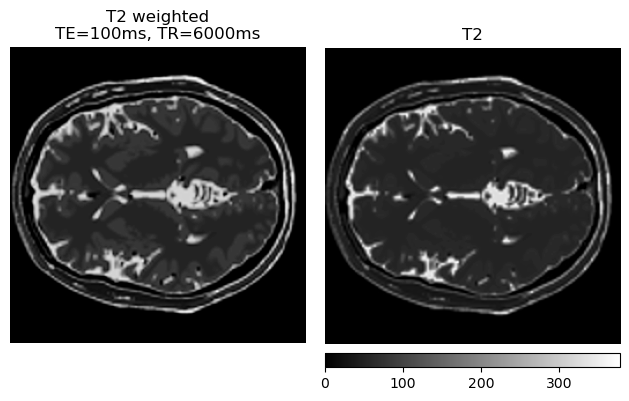
\includegraphics[width=0.8\textwidth]{figures/2_a_t2.png}
        \caption{Simulated T2 weighted SE image (left) compared to T2 map (right).}
        \label{fig:2_a_t2}
    \end{figure}

    \begin{figure}[]
        \centering
        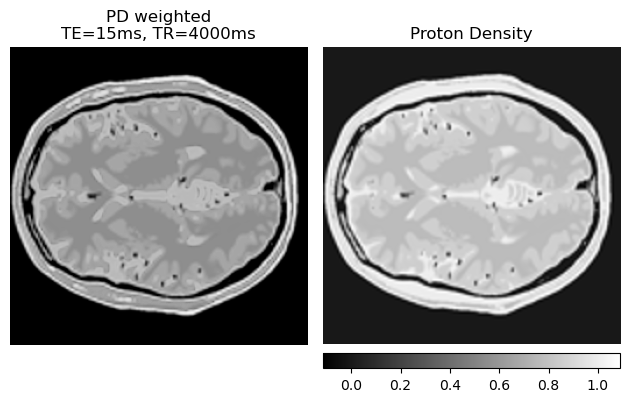
\includegraphics[width=0.8\textwidth]{figures/2_a_pd.png}
        \caption{Simulated PD weighted SE image (left) compared to PD map (right).}
        \label{fig:2_a_pd}
    \end{figure}

    \item[b. ] \textbf{Fast spin echo.}
    
    \begin{itemize}
        \item[ii.] I choose a k-space filling order where I group phase encoding lines which have been acquired at the same point in the echo train. With $ETL=32$, this results in 32 blocks of 8 k-space lines each. I fill k-space with these blocks and then shift them such that the block with $TE=TE_{eff}$ is in the center of k-space (cf. Figure \ref{fig:2_b_ii_kspace}). The resulting brain image with $ETL=32$, $TE_{eff}=80ms$ is shown in Figure \ref{fig:2_b_ii_image}.
        
        \begin{figure}[]
            \centering
            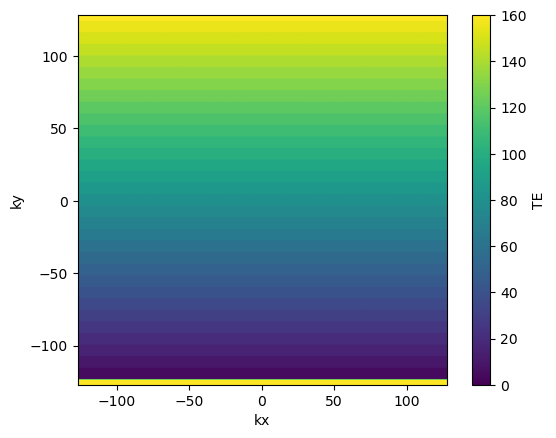
\includegraphics[width=0.8\textwidth]{figures/2_b_ii_kspace.png}
            \caption{k-space filling order for $ETL=32$, $TE_{eff}=80ms$.}
            \label{fig:2_b_ii_kspace}
        \end{figure}

        \begin{figure}[]
            \centering
            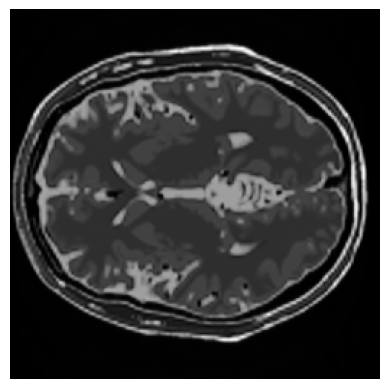
\includegraphics[width=0.7\textwidth]{figures/2_b_ii_image.png}
            \caption{Simulated FSE image for $ETL=32$, $TE_{eff}=80ms$.}
            \label{fig:2_b_ii_image}
        \end{figure}

    \end{itemize}
    

\end{itemize}

\end{document}